
%\documentclass[aspectratio=169]{beamer}
\documentclass{beamer}
\usetheme{Warsaw}
\usepackage{graphicx}
\usepackage{color}
\usepackage{listings}
\definecolor{dkgreen}{rgb}{0,0.6,0}
\definecolor{gray}{rgb}{0.5,0.5,0.5}
\definecolor{mauve}{rgb}{0.58,0,0.82}
\usepackage{amssymb}
\usepackage{amsthm}
\usepackage{amsmath}
\usepackage{amsopn}
\usepackage{hyperref}
\definecolor{codegreen}{rgb}{0,0.6,0}
\definecolor{codegray}{rgb}{0.5,0.5,0.5}
\definecolor{codepurple}{rgb}{0.58,0,0.82}
\definecolor{backcolour}{rgb}{0.95,0.95,0.92}
 \usepackage[version=4]{mhchem}
\lstdefinestyle{mystyle}{
    backgroundcolor=\color{backcolour},   
    commentstyle=\color{codegreen},
    keywordstyle=\color{magenta},
    numberstyle=\tiny\color{codegray},
    stringstyle=\color{codepurple},
    basicstyle=\footnotesize,
    breakatwhitespace=false,         
    breaklines=true,                 
    captionpos=b,                    
    keepspaces=true,                 
    numbers=left,                    
    numbersep=5pt,                  
    showspaces=false,                
    showstringspaces=false,
    showtabs=false,                  
    tabsize=2
}
\lstset{style=mystyle}
 \usepackage{pst-node,graphicx}
%\definecolor{mygreen}{RGB}{88, 102, 61}
\definecolor{myblue}{RGB}{51, 122, 153}
\definecolor{mygrey}{RGB}{ 216, 229, 215}
\definecolor{myred}{RGB}{198, 99, 59}
\definecolor{mywhite}{RGB}{255, 251, 244}
\definecolor{myolive}{RGB}{143, 163, 132}
\setbeamercolor{alerted text}{fg=orange}
\setbeamercolor{background canvas}{bg=mywhite}
\setbeamercolor{block title}{bg=myblue}
\setbeamercolor{normal text}{bg=mygrey,fg=black}
\setbeamercolor{palette sidebar primary}{use=normal text,fg=normal text.fg}
\setbeamercolor{palette sidebar quaternary}{use=structure,fg=structure.fg}
\setbeamercolor{palette sidebar secondary}{use=structure,fg=structure.fg}
\setbeamercolor{palette sidebar tertiary}{use=normal text,fg=normal text.fg}
\setbeamercolor{section in sidebar}{fg=brown}
\setbeamercolor{section in sidebar shaded}{fg=grey}
\setbeamercolor{separation line}{}
\setbeamercolor{sidebar}{bg=red}
\setbeamercolor{sidebar}{parent=palette primary}
\setbeamercolor{structure}{bg=black, fg=myblue}
\setbeamercolor{subsection in sidebar}{fg=brown}
\setbeamercolor{subsection in sidebar shaded}{fg=grey}
\setbeamercolor{title}{fg=white}
\setbeamercolor{titlelike}{fg=white}
\usepackage{epstopdf} 


\title{ Lunar Refueling Station}
\author{Leticia Damian \& Josh Lucas \& Rowan Ranjbar }
\institute[CSUSM] % (optional)
{
  \inst{1}%
  Dept. of Physics\\
  California State University San Marcos
}
 
\date % (optional){\today}

\begin{document}
 
\frame{\titlepage}


\begin{frame}{Goal of Project}
\begin{itemize}
\item Design a habitat that is suitable for habitation by at least two humans.\\
\item Maintain a stable temperature of $\approx 300K$
\item Protect from environmental hazards (Solar flux, cosmic rays...)
\item Generate power for air and water recycling and treatment.
\item Assume food can be initially supplied from rations sent from Earth
\end{itemize}

\end{frame}


\begin{frame}{Location of Habitat}
  The location of the base must then take in to account proximity to probable water locations as well as areas of illumination for solar power and heat generation as well as line of sight for communication.
\end{frame}


\begin{frame}{Location of Habitat}
      \begin{center}
             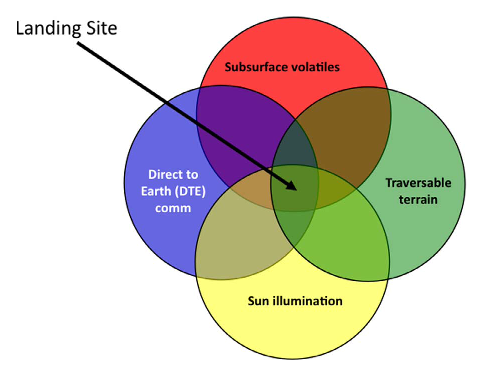
\includegraphics[width= .75\textwidth]{site.eps}   
      \end{center}  
     Acesss to water, ilumination, communication, and mobility. \cite{Heldmann}
\end{frame}

\begin{frame}{Why the lunar Poles}
 
 The moon resides along the elliptical plane. As a result the poles receive much less light than the lower latitudes. There are craters on the moon then that are permanently shadowed regions or \textbf{PSR}s. There are also highlands that remain permanently illuminated (\textbf{PIR}s).
 \begin{center}
             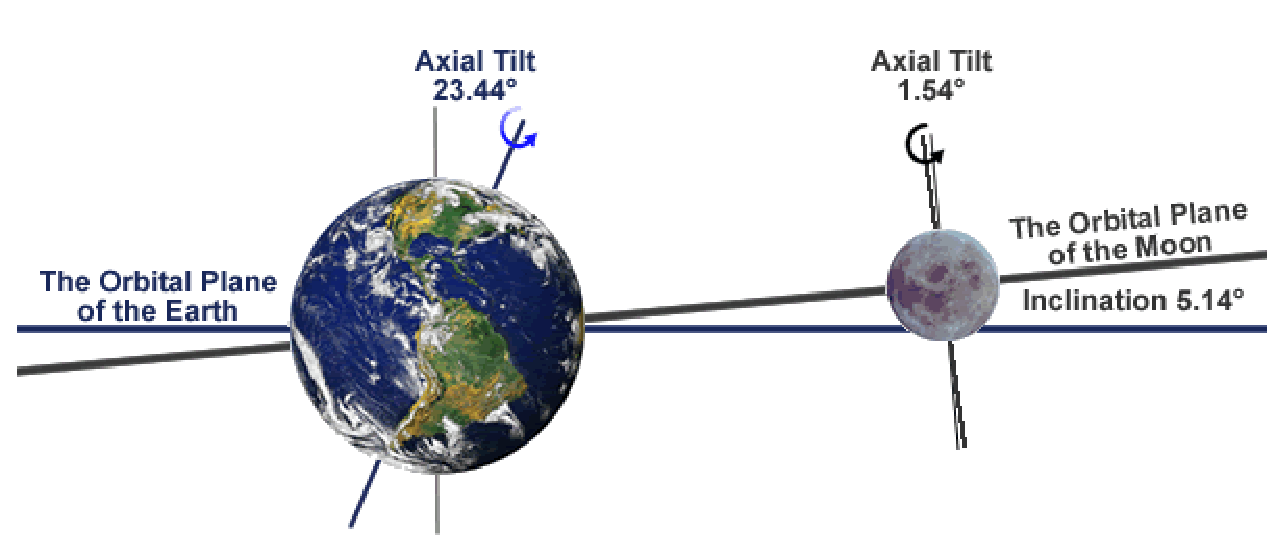
\includegraphics[width= 1\textwidth]{earth-moon.eps}   
      \end{center}  
\end{frame}

\begin{frame}{Temperatures at the Lunar Southern Pole}

The Shackleton crater at the lunar south pole is a highly researched area for habitation. The temperature varies from a high of $213K $ and a low of $50K$
\cite{Williams}.
 \begin{center}
             \includegraphics[width= 1\textwidth]{SouthTemp.eps}   
      \end{center}  
\end{frame}

%
%\begin{frame}{Habitat}
%To support human life the habitat needs to maintain a temperature of approximately 300K as well as protect from bombardment of radiation and micro meterors. (include radiation levels , sources, meteors)
%\end{frame}


\begin{frame}{Illumination at the Lunar South Pole}
       \begin{columns}
          \column{0.70\linewidth}
             \centering
             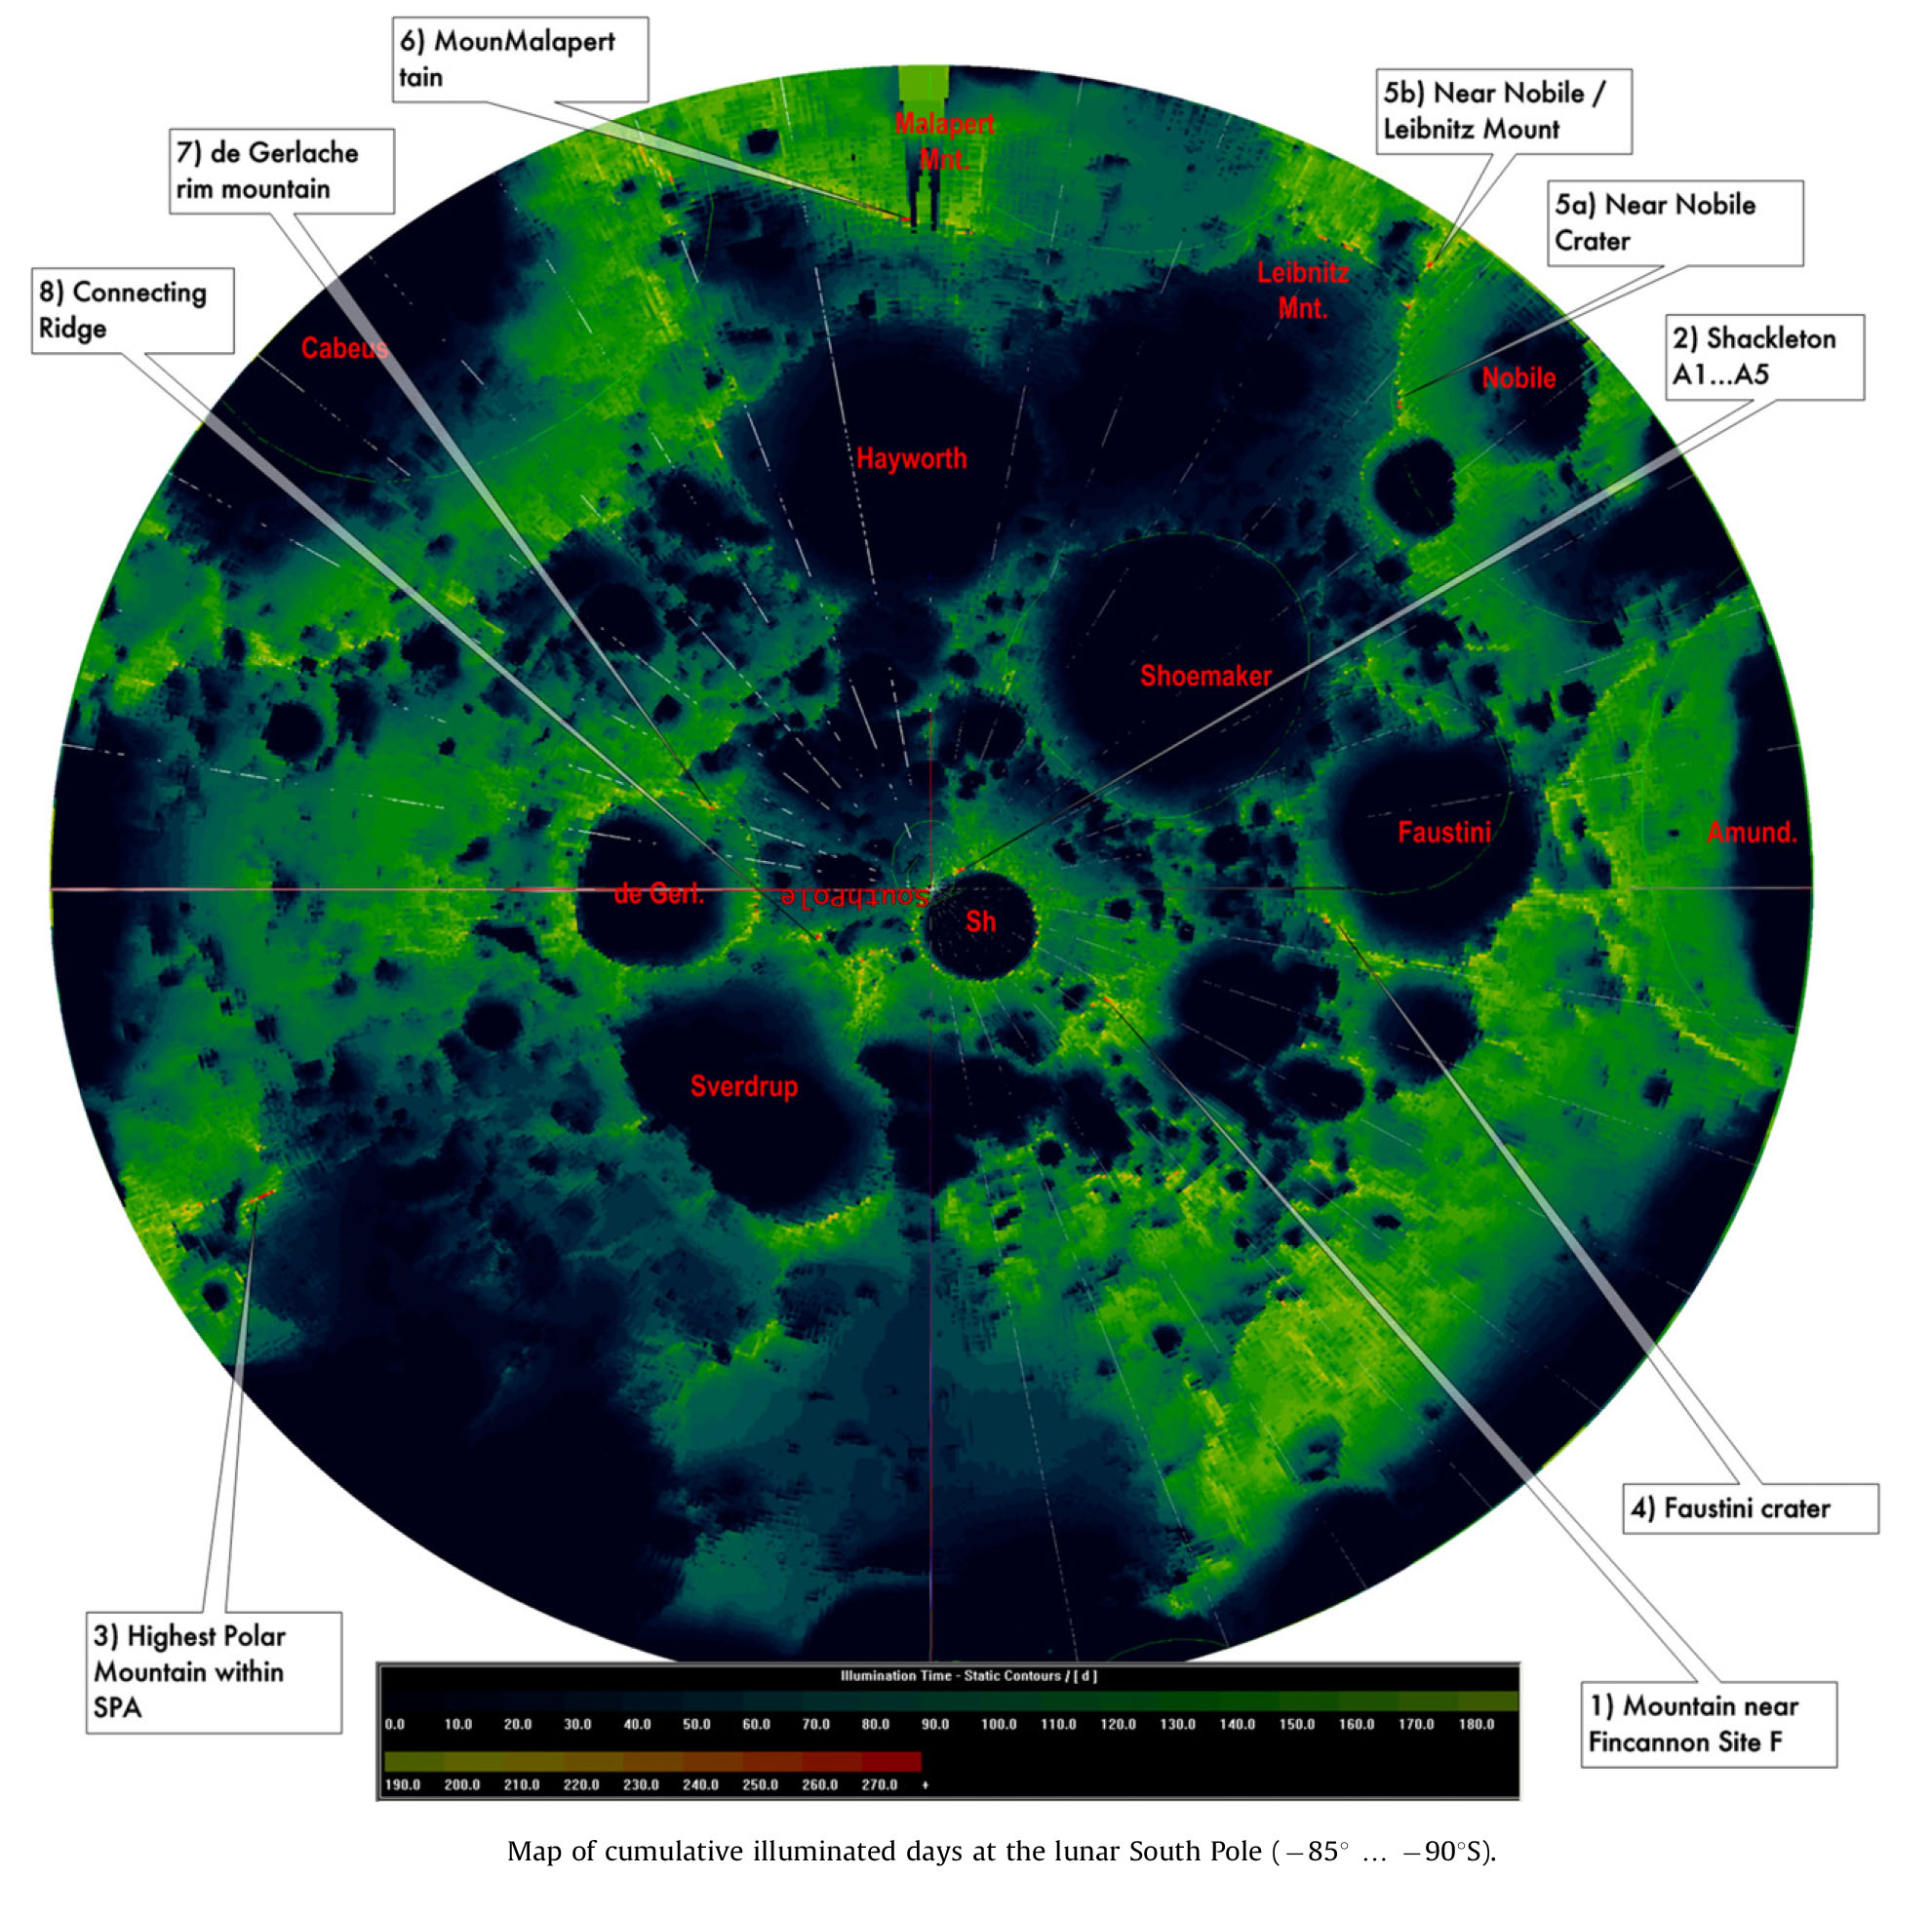
\includegraphics[width= \textwidth]{South_Pole_Light.jpg}
           \column{0.30\linewidth}
            The incident angle of sunlight rotates by $360^{\circ}$ over a month period.\\
            The further from the center of the pole the higher a solar collector would need to be recieve maximum illumination.  \cite{Koebel}
         \end{columns} 
    \end{frame}


\begin{frame}{Power Demands}
Each inhabitant at a minimum will require 3kWe. Photovoltaic arrays have been extensivly and reliable used in space and surface explorations. PV systems will require energy storage systems for times of little to no illumination. Nuclear power would provide continuous power but present several saftey and political barriers to become feasible\cite{Hickman}.
\end{frame}

\begin{frame}{Solar-Thermal Power Generation}
       \begin{columns}
          \column{0.65\linewidth}
             \centering
             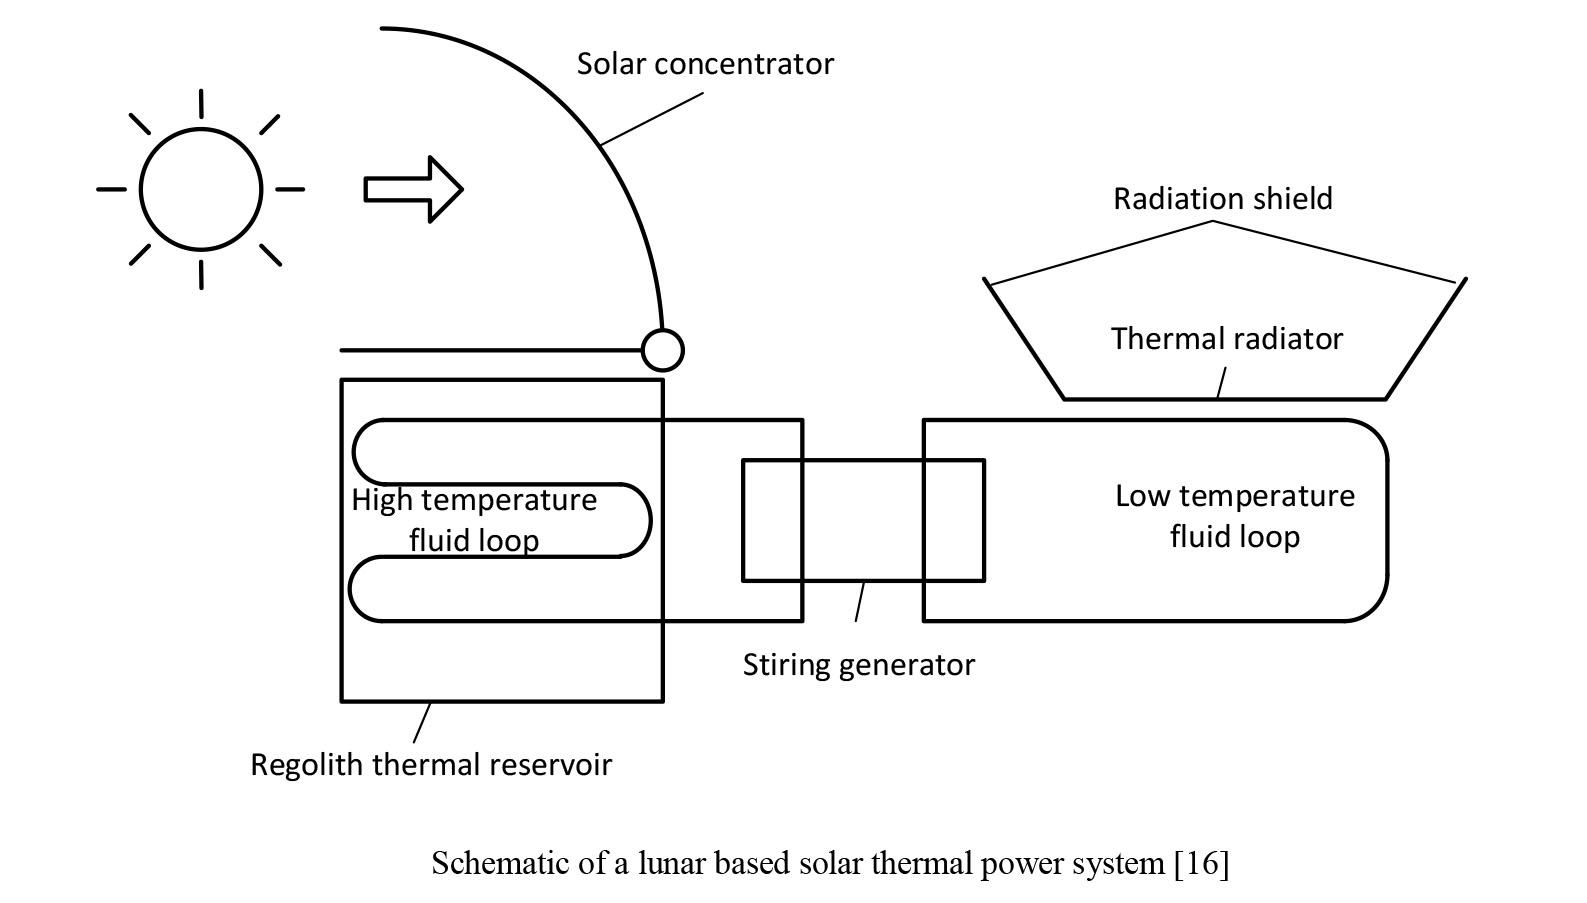
\includegraphics[width= \textwidth]{Solar_thermal.jpg}
           \column{0.35\linewidth}
              The Stirling generator converts the
thermal energy stored in lunar regolith into electrical power.\cite{Yao}\cite{Climent}
         \end{columns} 
         \center
         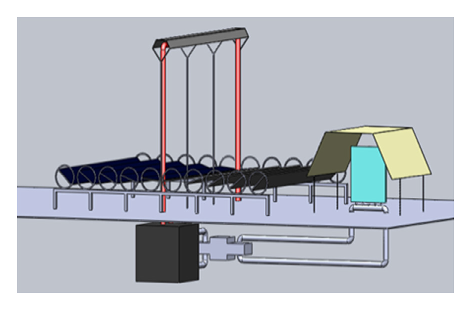
\includegraphics[width= .5\textwidth]{Heat_night.eps}
    \end{frame}



\begin{frame}{Insulating and Protective Barrier }
The moon regolith itself can be used as shielding and insulating material to protect against extreme temperatures and frequent micro-meteorite bombardment (10-30Km/s) as well as solar flares and cosmic radiation.
\cite{Toth}
\center
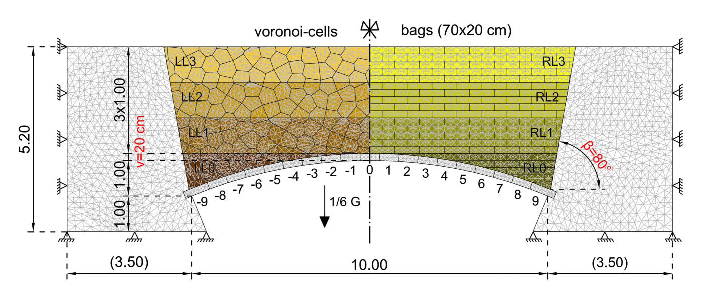
\includegraphics[width= .95\textwidth]{bags.eps}   
\end{frame}

 

    
    
  \begin{frame}{Food, Oxygen, and Water needs}
      \begin{center}
             
\includegraphics[width= \textwidth]{Human_needs.eps}   
      \end{center}  
              Life Support Systems (LSS) need effecient managament of Oxygen, food, water, and saftey.\cite{Belz}

    \end{frame}











\begin{thebibliography}{99}
% The numeral (here 99) in curly braces is nominally the number of entries in
% the bibliography. It's supposed to affect the amount of space around the
% numerical labels, so only the number of digits should matter--and even that
% seems to make no discernible difference.



\bibitem{Koebel}David Koebel, Michele Bonerba, Daniel Behrenwaldt, Matthias Wieser, Carsten Borowy,
Analysis of landing site attributes for future missions targeting the rim of the lunar South Pole Aitken basin,
Acta Astronautica,
Volume 80,
2012,
Pages 197-215

\bibitem{Yao}Xiaochen Lu, Wei Yao, Chao Wang, Rong Ma,
Exergy analysis of a lunar based solar thermal power system with finite-time thermodynamics,
Energy Procedia,
Volume 158,
2019,
Pages 792-796


\bibitem{Belz} Belz et al., 2011. Hybrid life support systems with integrated fuel cells and photobioreactors for a lunar base. Aerospace Science and Technology, pp.Aerospace Science and Technology.

\bibitem{Hickman}Hickman, J.M., Curtis, H.B. \& Landis, G., 1990. Design considerations for lunar base photovoltaic power systems, Washington, DC] : [Springfield, Va.]: National Aeronautics and Space Administration

\bibitem{Climent}Blai Climent, Oscar Torroba, Ricard González-Cinca, Narayanan Ramachandran, Michael D. Griffin,
Heat storage and electricity generation in the Moon during the lunar night,
Acta Astronautica,
Volume 93,
2014,
Pages 352-358

\bibitem{Heldmann}Jennifer L. Heldmann, et al. Site selection and traverse planning to support a lunar polar rover mission: A case study at Haworth Crater,
Acta Astronautica, Volume 127, 2016, Pages 308-320,

\bibitem{Toth}Toth, A.R. \& Bagi, K., 2011. Analysis of a Lunar Base Structure Using the Discrete-Element Method. Journal Of Aerospace Engineering, 24(3), pp.397–401.

\bibitem{Williams}J.P. Williams, D.A. Paige, B.T. Greenhagen, E. Sefton-Nash,
The global surface temperatures of the Moon as measured by the Diviner Lunar Radiometer Experiment,
Icarus,
Volume 283,
2017,
Pages 300-325

\end{thebibliography}


\end{document}